\documentclass[12pt,a4paper]{article}

\setlength{\parindent}{0.1 in}
%\setlength{\parskip}{0.1 in}
\setlength{\oddsidemargin}{0.25 in}
\setlength{\evensidemargin}{-0.25 in}
\setlength{\topmargin}{-0.5 in}
\setlength{\textwidth}{7.0 in}
\setlength{\textheight}{9.5 in}
\setlength{\headsep}{0.45 in}

%\usepackage[fleqn]{amsmath}
%\usepackage{amsfonts,graphicx}
\usepackage{amsmath,amsfonts,graphicx}
\usepackage[fleqn]{mathtools}
\usepackage{setspace}
\usepackage[colorlinks=false, pdfborder={0 0 0}]{hyperref}
\usepackage[nottoc]{tocbibind}
\usepackage{tocloft}
\usepackage[outermargin=2 in]{geometry}
\usepackage{scrextend}
\usepackage{tensor}
\usepackage{cancel}
\usepackage{slashed}


%Adding `Appendix' to the appendices
\usepackage[toc,page]{appendix}

%Add a bullet point to description items
\usepackage{enumitem}

%Mathematics
\usepackage{braket}
\usepackage{ulem}
\usepackage{xcolor}
\usepackage[font={small,it}]{caption}

\bibliographystyle{unsrt}

% Packages that Gavin uses
\usepackage{url}
\usepackage[font=footnotesize]{caption}
\usepackage[font=footnotesize]{subcaption}
\usepackage[]{microtype}
\usepackage{balance}
\usepackage{cite}
\usepackage{lmodern}
\usepackage[T1]{fontenc}
\usepackage{doi}

% Nice typesetting of SI units
\usepackage{siunitx}
\sisetup{range-phrase=--}
\sisetup{separate-uncertainty = true}

% SImons packages
\usepackage{float}



%New commands
%Maths
\newcommand{\beq}{\begin{equation}}
\newcommand{\eeq}{\end{equation}}
\newcommand{\bea}{\begin{align}}
\newcommand{\eea}{\end{align}}
\newcommand{\p}{\partial}
\newcommand{\trace}[1]{\mathrm{Tr}\left[#1 \right]}
\newcommand{\ptrace}[2]{\mathrm{Tr}_{#1} \left[ #2 \right]}
\newcommand{\bpmat}{\begin{pmatrix}}
\newcommand{\epmat}{\end{pmatrix}}
\newcommand{\vv}[1]{\mathbf{#1}}
\newcommand{\mat}[1]{\uuline{#1}}
\newcommand{\norm}[1]{\| #1 \|}
\newcommand{\op}[1]{\mathbb{#1}}
\newcommand{\vhat}[1]{\hat{\vv{#1}}}

%Renewed commands, in order for them to take arguments with automatically adjusted brackets 
\renewcommand{\dim}[1]{\mathrm{dim}\left( #1\right)}
\renewcommand{\det}[1]{\mathrm{det} \left( #1 \right)}
\renewcommand{\exp}[1] {\mathrm{exp} \left[ #1 \right]}


%\mathbb Letters
\newcommand{\identity}{\mathbb{I}}
\newcommand{\inreal}{\mathbb{R}}
\newcommand{\incomplex}{\mathbb{C}}

%Redefine Braket
\renewcommand{\braket}[1]{\left\langle #1 \right\rangle}

%Integration
\newcommand{\intd} {\mathrm{d}}

%Operators
\newcommand{\phihat}{\hat{\phi}}
\newcommand{\xhat}{\hat{x}}
\newcommand{\phat}{\hat{p}}
\newcommand{\Dhat}{\hat{D}}
\newcommand{\Hhat}{\hat{H}}
\newcommand{\ahat}{\hat{a}}
\newcommand{\bhat}{\hat{b}}
\newcommand{\chat}{\hat{c}}
\newcommand{\Phihat}{\hat{\Phi}}

%Channels
\newcommand{\channel}[3]{\mathcal{#1}^{#2 \rightarrow #3}}


%Caligraphy letters
\newcommand{\cl}[1]{\mathcal{#1}}
\newcommand{\Hilbert}{\mathcal{H}}
\newcommand{\calN}{\mathcal{N}}
\newcommand{\Lag}{\mathcal{L}}
\newcommand{\calD}{\mathcal{D}}


%Pauli
\newcommand{\Xhat}{\hat{X}}
\newcommand{\Yhat}{\hat{Y}}
\newcommand{\Zhat}{\hat{Z}}
\newcommand{\PauliX}{\bpmat 0 & 1 \\ 1 & 0 \epmat}
\newcommand{\PauliZ} {\bpmat 1 & 0 \\ 0 & -1\epmat}



%Gell-Mann matrices
\newcommand{\GMone} {\bpmat 0 & 1 & 0 \\ 1 & 0 & 0 \\ 0 & 0 & 0 \epmat }
\newcommand{\GMsix}{\bpmat 0 & 0 & 0 \\ 0 & 0 & 1\\ 0 & 1 & 0\epmat}

%Density matrices
\newcommand{\rhotwo}{\bpmat 1 & e^{-it} \\ e^{it} & 1 \epmat}
\newcommand{\rhothree} {\bpmat 1 & e^{it} & e^{2it} \\
e^{-it} & 1 & e^{it} \\
e^{-2it} & e^{-it} & 1 \epmat}



%Misc
\def\dbar{{\mathchar'26\mkern-12mu d}} %a $d$ with a bar through its stem


\newcommand{\eq}[1]{$#1$}

%Undertilded quantities
\newcommand{\tildeq}{\underset{^\sim}q}
\newcommand{\tildep}{\underset{^\sim}p}

%Curly letters
\newcommand{\calE}{\mathcal{E}}

\newcommand{\Nhat}{\hat{N}}

%Wave vector shortening
\newcommand{\kvec}{\vv{k}}













\usepackage{url}
\usepackage{amsmath}
\usepackage{graphicx}
\usepackage[font=footnotesize]{caption}
\usepackage{subcaption}
\usepackage[]{microtype}
\usepackage{balance}
\usepackage{cite}
\usepackage{braket}
\usepackage{braket}
\usepackage{siunitx}

\begin{document}
\title{Summary of work}
\author{Gavin Dold, Sofia Qvarfort, Simon Schaal}
\maketitle
\tableofcontents
\section{Introduction}
We have simulated a probe qubit interacting with four data qubits. 


\section{Dephasing}
In this section, we present results from simulations of the Lindblad master equation where a dephasing channel is turned on. This channel contains the Lindblad operator
\beq
L  = \sqrt{\Gamma} \sigma_z
\eeq

where $\Gamma$ is the dephasing parameter, which is also $1/\tau$ where $\tau$ is the dephasing time. 

We evolve the system under the Lindblad master equation for an odd number of errors. This causes the final phase of the probe qubit to end up at $\phi = \pi$. 

In Figure \ref{fig:BlochsphereDephasing}, we see the effect of a small dephasing coefficient (100) whereas in Figure \ref{fig:somethig} we see the effect of larger dephasing (500). Note that the dephasing happens primarily as the interaction between the probe qubit and the data qubit is weak. 



\begin{figure}[!ht]
  \caption{A picture of a gull.}
  \centering
    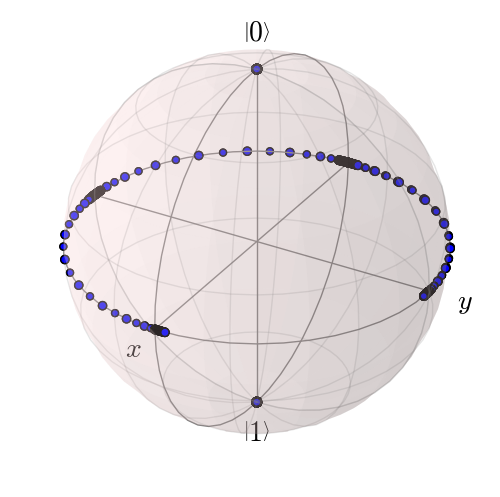
\includegraphics[width=\textwidth]{Figures/Circ_orbit_odd_no_dephasing.png}
\end{figure}




\begin{figure}[!ht]
  \caption{A picture of a gull.}
  \centering
    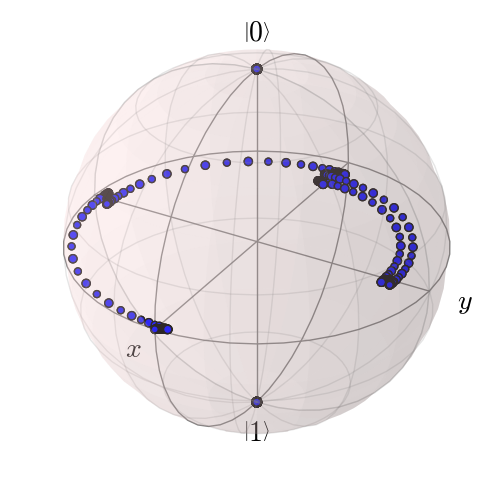
\includegraphics[width=\textwidth]{Figures/Circ_orbit_odd_100_dephasing.png}
\end{figure}

In Figure \ref{fig:plot} we see the effect of dephasing on the probability of measuring the correct value of the probe qubit. Since there is an odd number of errors, we want the probe qubit to end up in the $\ket{-}$ state. However, the dephasing will cause the probe qubit to become a mixed state $\rho$, for which we have a finite probability of measuring $\ket{+} $ instead of $\ket{-}$. For complete dephasing, the probe qubit becomes a mixed state which has a 50-50\% chance of measuring either state. 

In Figure \ref{fig:Plot}, we have market the data-point for dephasing corresponding to the decoherence time for Bismuth, which is one of the proposed donor types for the probe qubit. The decoherence time of bismuth is 2.7 s \cite{something}, which leads to a dephasing parameter of 0.37 s$^{-1}$. 

\begin{figure}[!ht]
  \caption{A picture of a gull.}
  \centering
    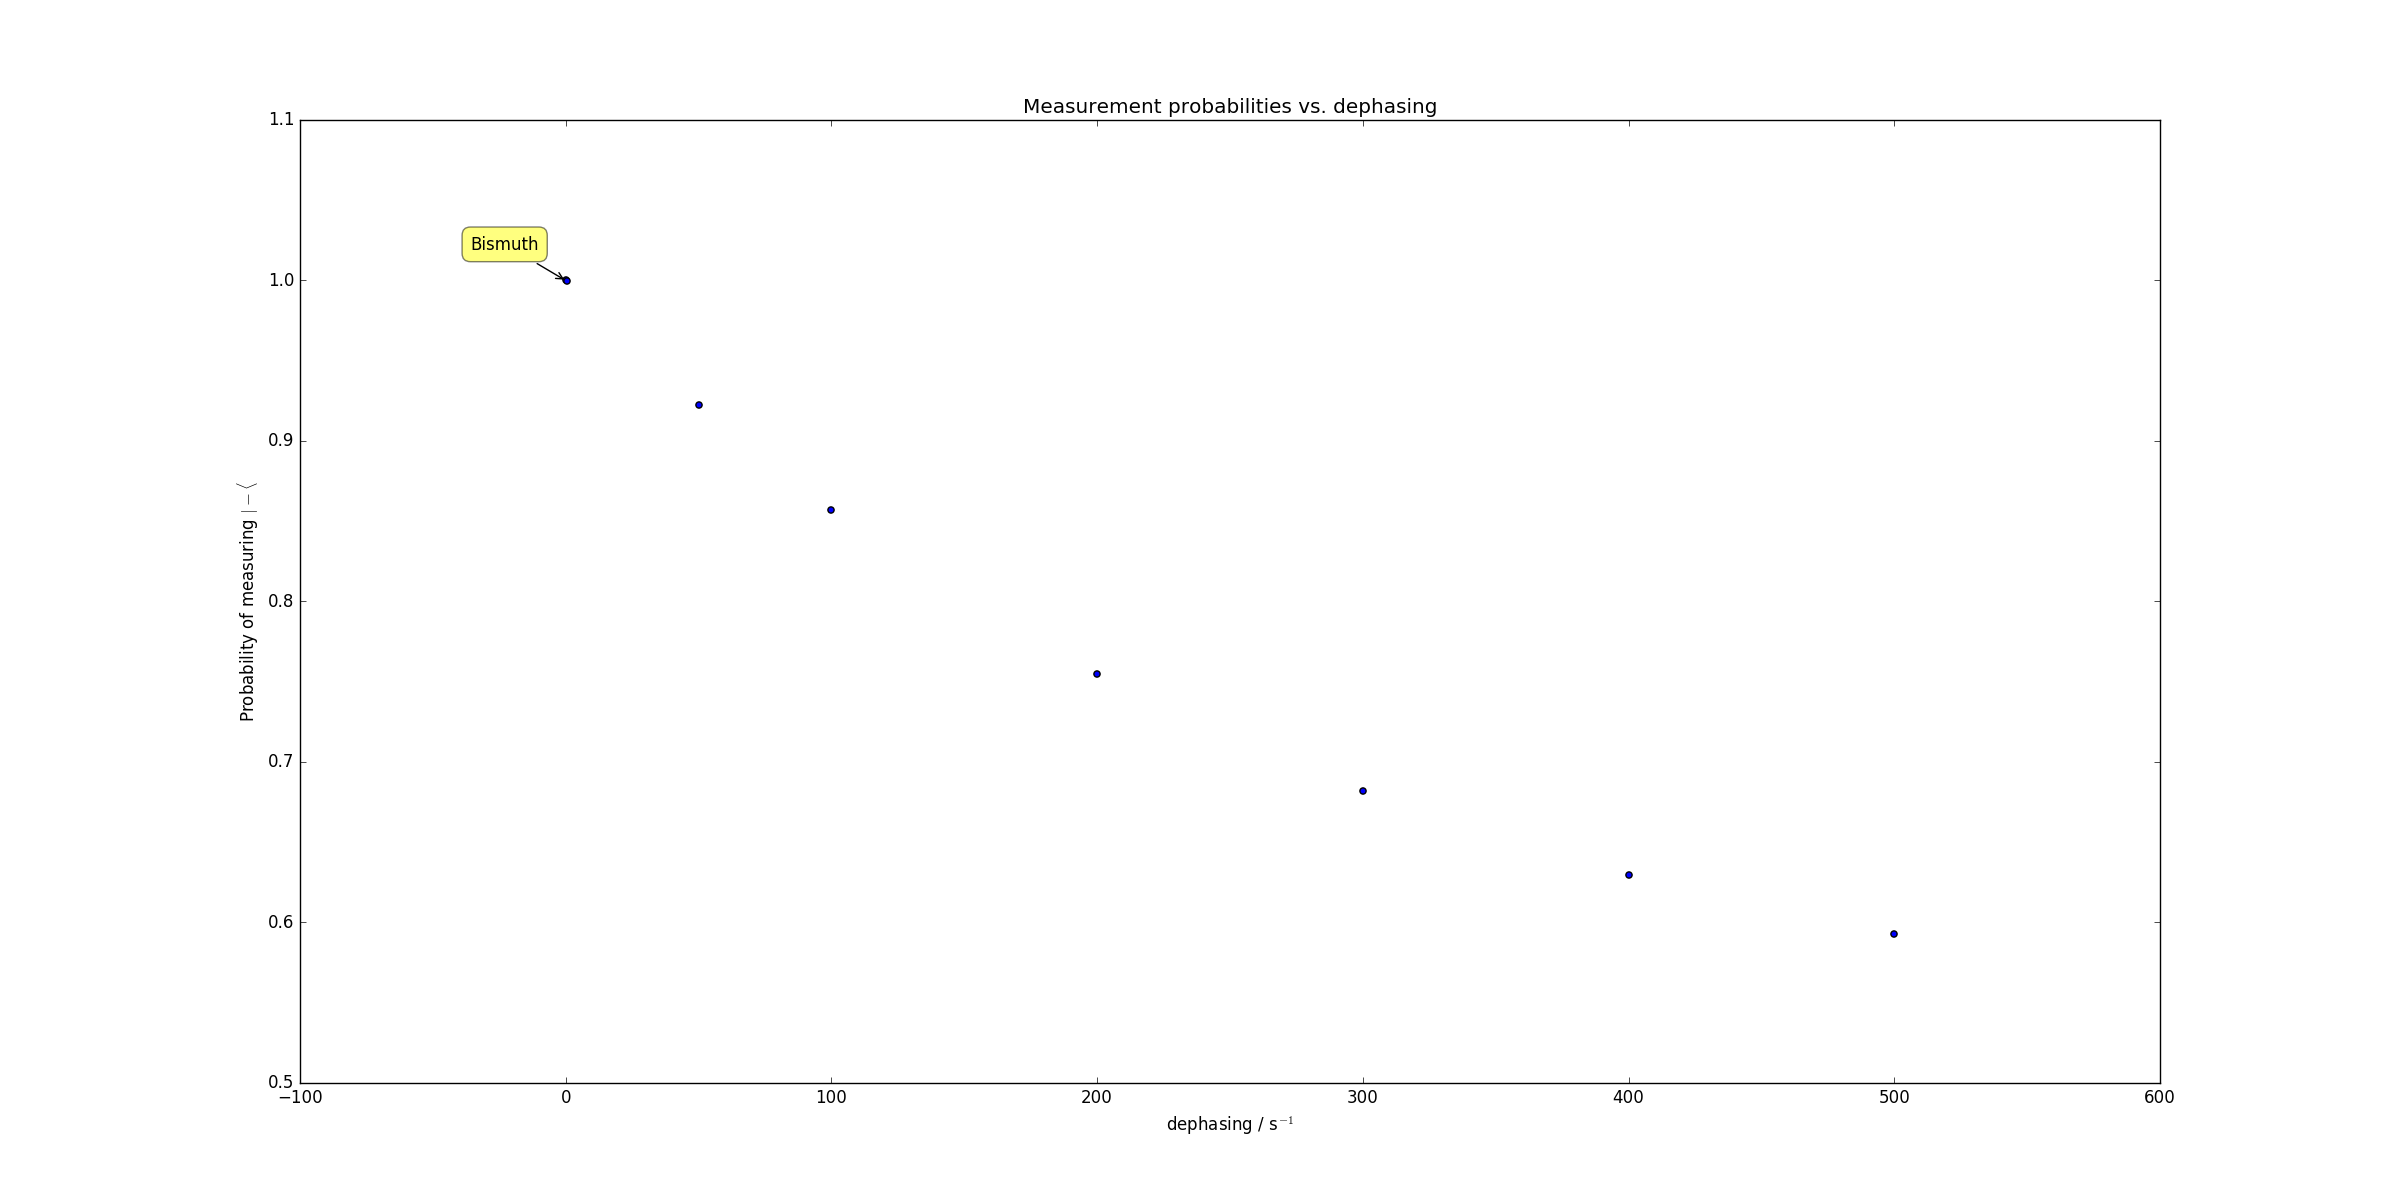
\includegraphics[width=\textwidth]{Figures/measurement_dephasing_graph.png}
\end{figure}

\section{Dopant Placement}
\begin{figure}
	\centering
	\begin{subfigure}[t]{0.7\textwidth}
		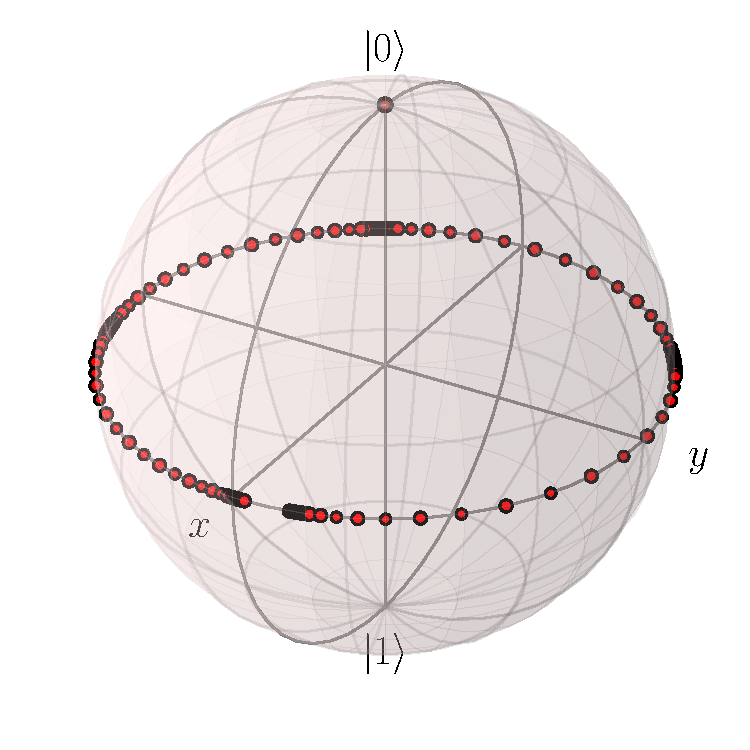
\includegraphics[width=\textwidth]{figures/z_offset.pdf}
		\caption{Evolution of probe qubit with data qubit displacement in the Z direction. 1st and 2nd qubits are displaced \SI{4}{\nano\metre} down, slowing the evolution, the 4th is displaced \SI{3}{\nano\metre} up with a resultant increase in phase accumulated. The overall deviation from $2\pi$ is small as a result.}
		\label{fig:zoffset}
	\end{subfigure}
	\begin{subfigure}[t]{0.7\textwidth}
		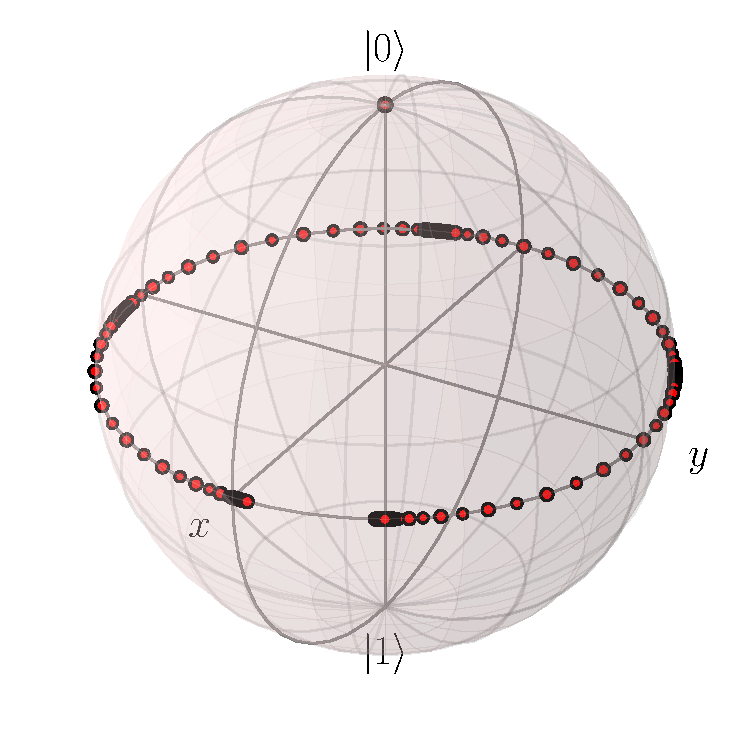
\includegraphics[width=\textwidth]{figures/10nm_displacement_inward.pdf}
		\caption{Phase accumulated when all 4 data qubits are displaced \SI{10}{\nano\metre} towards the centre of the circle. Other directions of \SI{10}{\nano\metre} displacements result in similar phase deviations.}
		\label{fig:inwarddisplacement}
	\end{subfigure}
	
	\caption{Phase errors as a result of misplaced data qubits.}
	\label{fig:overall_displacement}
\end{figure}

\section{Path Jitter}


\end{document}